%%%%%%%%%%%%%%%%%%%%%%%%%%%%%%%%%%%%%%%%%%%%%%%%%%%%%%%%%%%%%%%%%%%%%%%%%%%%%%%%%%%%%%%%%%%%%
%%									Chapitre 5                      						  % 
%%%%%%%%%%%%%%%%%%%%%%%%%%%%%%%%%%%%%%%%%%%%%%%%%%%%%%%%%%%%%%%%%%%%%%%%%%%%%%%%%%%%%%%%%%%%%
	
\renewcommand{\tablename}{Tableau}
\renewcommand{\figurename}{Figure}
%\newcommand{\corriger}[1]{\textcolor{red}{#1}}
\newcommand{\sncom}[1]{{\color{black}{\textsf{[para  #1]}}}}
\newcommand{\sncomc}[1]{{\color{Blue}{\textsf{[com :  #1]}}}}
\chapter{Conclusions et perspectives} \label{chapter_5}
	
	\minitoc
	\newpage
		
\section{Modélisation et calibration}
	Dans cette thèse, nous avons proposé un modèle semi-discret décrivant la dynamique de racines des plantes et des nématodes au sein et entre les saisons de
cultures.  À partir d’un modèle  épidémiologique simple,  nous avons pu  décrire la dynamique d’infection d’une plante saine par
des nématodes sur une saison. L’ajustement des paramètres de notre modèle à des données expérimentales disponibles dans la littérature \citep{Ehwaeti1998} nous a permis de
reproduire assez fidèlement la croissance de la plante infectée par les nématodes. Nous avons  réitéré cette démarche sur nos propres données expérimentales (section~\ref{sec:experimentation}  et \Cref{secanchap4}). Le modèle s'est très bien ajusté  aux données expérimentales de cette seconde expérimentation (voir \ref{sec:résultats-chapitre4}.\autoref{sec:calibration}).  Cette étude permet ainsi de montrer que notre modèle mécaniste peut représenter des conditions expérimentales très différentes grâce à des réajustements des valeurs des paramètres. En outre, les valeurs des paramètres estimées à partir des deux expériences sont globalement comparables (voir  \autoref{comp:para}), en particulier le taux d'infection qui a un fort impact sur les sorties de notre modèle.  Ce résultat nous permet d'être plus confiants sur la valeur des paramètres inconnus que nous avons utilisés dans cette étude et renforce les conclusions du \autoref{article}.
	  
	Notre  modèle est donc suffisamment  générique pour  s'adapter à différentes interactions plantes--nématodes.
Pour cela, il faut estimer   les paramètres spécifiques à la plante, au nématode et au contexte cultural ou agronomique considéré. Par exemple pour  la plante, il faut calibrer  la masse initiale et le taux de croissance des racines. Chez le nématode, il faut  estimer le taux de contamination, le taux de reproduction, les coûts de fitness, \textit{etc}.   Avec des modifications mineures, notre modèle pourrait  également s'adapter à d'autres pathogènes ou bioagresseurs telluriques (champignons, virus, bactéries).   On pourrait par exemple prendre en compte les infections secondaires qui sont caractéristiques de nombreux pathosysthèmes impliquant les parasites telluriques de plantes  \citep{Cunniffe2011,Mailleret2012}. A l'avenir, nous espérons que ce type de modèle contribuera à une plus grande
considération du rôle des processus biologiques et évolutifs dans le cadre de la modélisation de la dynamique d'interaction  hôte--parasite.
	
	     
	Pour notre étude, nous disposions de trois points de mesures dans le temps pour suivre l'infection de tomates par les nématodes (42  et 135 jours post-inoculation pour l'expérience de \citet{Ehwaeti1998} et 35 jours pour notre expérimentations). Il serait intéressant d'acquérir davantage de données de suivis temporels, afin d'avoir une meilleure vision de la dynamique d'infestation. 
Il s'agirait par exemple de mettre en place une expérience en serre permettant de mesurer les densités de nématodes dans le sol et dans les racines (les pontes, indices de galles) régulièrement (par exemple toutes les deux semaines)  sur  un cycle de culture. Une  telle expérience  nécessiterait un grand nombre de plants et de nématodes, car toutes ces mesures sont destructives. Elle engendrerait également un travail de suivi et de mesure conséquent. C'est sans doute ce qui explique le peu de données de ce type rencontrées dans la littérature.
	 
	Obtenir de nouvelles  données pour des cultures d'espèces différentes de la tomate (\textit{e.g.} melon, poivrons, salades)  permettrait d'autre part d'enrichir notre modèle et d'ouvrir vers d'autres perspectives également très intéressantes comme la rotation d'espèces plutôt que la rotation de variétés. La calibration  de notre modèle pour différentes espèces de cultures intra-saisonnières  (culture de cucurbitacées ou solanacées) et  inter-saisonnières permettrait d'avoir une modélisation plus pertinente des rotations  de cultures  pratiquées chez les agriculteurs du sud de la France. 
Par exemple, de plus en plus d'agriculteurs ont un intérêt marqué pour les systèmes de cultures du projet  \gls{GEDUNEM}, qui montre que la combinaison de pratiques agronomiques avec la rotation de différentes espèces hôtes de plantes  améliorent l’efficacité du contrôle des nématodes et la durabilité des méthodes de lutte exploitant les \glspl{gene R} aux nématodes \citep{Djian-Caporalino2019}. 
	 
	 Enfin, outre les données expérimentales utilisées dans cette thèse, nous pourrions acquérir de nouvelles données (\textit{e.g.} nombre et taille des fruits) pour quantifier l'impact des nématodes sur la production végétale, ou encore l'effet des  pratiques agriculturales, comme la solarisation ou l'utilisation de mauvais hôtes, de plantes
biofumigantes ou de plantes  pièges (données en partie présentes dans \gls{GEDUNEM}).
	
\section{Les critères d'optimisation}
	
\subsection{L’intérêt de notre critère}
	
	Dans cette étude, nous cherchons à maximiser le rendement moyen saisonnier d'une plante. Nous approximons le rendement saisonnier  par la densité de racines saines cumulée au cours du temps. C'est le pendant en surface \og verte\fg{} ou saine de l'\glsname{AUDPC} (\og area under the disease progress curve\fg{}). Ce critère est assez simple et est largement utilisé en épidémiologie végétale \citep{Jeger2004, Rimbaud2018}, y compris pour un pathosystème impliquant un autre nématode des racines \citep{Tankam-Chedjou2020}. 
Cette quantité est similaire à la durée de la surface foliaire saine ($HAD$),
l'intégrale de la surface des feuilles saines pendant une saison de croissance,
utilisée par de nombreux auteurs pour les pathogènes aériens \citep{Waggoner1987,Gooding2000,vandenBosch2003,LoIacono2012,Elderfield2018,Papaix2018}.
	 
\subsection{Les améliorations possibles}
	
	Notre critère d'optimisation se heurte à certaines limitations :  1) c'est une approximation certes courante, mais néanmoins assez grossière du rendement total  de la plante ; 2) l'optimisation de ce critère génère une forte variabilité temporelle du rendement ;  3) ce critère ne permet pas d'optimiser  de manière explicite la durabilité  des gènes majeurs de résistance.
	
	Premièrement,  nous pourrions améliorer le proxy que nous avons utilisé pour le rendement des cultures en représentant les interactions entre racines et croissance des fruits. Un couplage de notre modèle épidémiologique avec un modèle écophysiologique prenant en considération les parties végétative et racinaire de la plante, à l'instar des travaux de Valentina Baldazzi qui travaille dans notre équipe M2P2 et en collaboration avec l'équipe IPN,  permettrait de passer à un rendement plus pertinent pour de futures investigations. Des premiers résultats intéressants ont été obtenus lors d'un stage de Master 2 \citep{Breniere2018}.
	
	Deuxièmement, nous pourrions améliorer ou modifier notre critère de différentes manières pour pallier la forte variabilité temporelle du rendement, induite par les
rotations entre  cultures résistantes et  sensibles. Par exemple, nous
pourrions définir un seuil de rendement satisfaisant économiquement et pénaliser dans notre critère toutes les rotations menant à des rendements annuels plus bas que ce seuil.
Tout en maximisant le rendement, nous pourrions aussi minimiser la variance du rendement, afin d'assurer des revenus stables aux agriculteurs. 
	
	Troisièmement, la maximisation du rendement, même avec des rotations alternant plantes résistantes et sensibles, n'a pas pour objectif d'optimiser la durabilité de la résistance des plantes.
Un critère visant à préserver la durabilité tout en utilisant le potentiel de la résistance pour réduire les dégâts engendrés par les nématodes, pourrait par exemple consister à maximiser le rendement moyen saisonnier sous la contrainte de ne pas dépasser un seuil de nématodes virulents (90\% par exemple, comme proposé par \citet{vandenBosch2003}}). \citet{Fabre2015}, grâce à un critère quasi-similaire,  ont déterminé des stratégies optimales maximisant le rendement tout en préservant la durabilité des résistances des plantes.  Par ailleurs, on pourrait aussi utiliser un critère visant à maximiser le rendement des cultures au cours des saisons de culture et à minimiser la proportion de virulents à la fin de l’horizon temporel. Cela permettrait de ne pas recourir massivement au déploiement de la résistance lors des dernières saisons considérées, ce qui pourrait mener à un contournement massif de la résistance peu après la fin de cet horizon temporel.
	
\selectlanguage{french} %ou english
	
\section{La résistance des plantes aux nématodes}
	
\subsection{Gènes majeurs tardifs et précoces} \label{sec:compR-resistance-precoce-tardive}
	
	 Dans la famille des \textit{Solanaceae}, il existe deux types de \glspl{gene R}
	avec différents modes d'action : le gène \textit{Me3} du piment, comme le gène \textit{Mi-1} de la tomate, engendrent une \gls{HR} précoce lorsque le nématode pénètre dans le système racinaire ; le gène  \textit{Me1}, qui lui engendre une \gls{HR} tardive lorsque le nématode crée son site nourricier \citep{Castagnone-sereno2001,Pegard2005, Djian-Caporalino2011}. 
Dans le \autoref{article},  nous nous sommes basés sur le gène \textit{Mi-1} de la tomate. Cependant, nous avons vu que la résistance tardive est plus durable que la résistance précoce (section~\ref{sec:gene-R-piment}.\ref{sec:mécanisme-contournement}). Une des hypothèses concernant la plus grande durabilité de ce \gls{gene R} serait liée au fait que les réactions de défense provoquées plus profondément dans la racine bloqueraient irréversiblement le développement de tout autre nématode, empêchant ainsi la sélection d'un génotype virulent. 
	
	Nous avons ainsi mené une étude préliminaire pour comparer ces deux types de \glspl{gene R}. Nous avons tout d'abord comparé le déploiement optimal de chaque plante résistante en alternance avec une plante sensible, en utilisant le critère fondé sur le rendement en section~\ref{sec:hrd}. Pour cela, nous avons utilisé deux versions de notre modèle d'interactions plante--nématodes : celle présentée en \ref{sec:introduction-virulents}.\autoref{sec:model-resistance-precoce} correspondant à une résistance précoce et une version avec un gène de résistance tardif, qui induit une \og immunité \fg{} de la plante. Dans ce dernier modèle, nous supposons qu'un nématode avirulent peut pénétrer dans la racine d'une plante avec résistance tardive, mais qu'il est bloqué avant l'initiation de son site nourricier ; une fraction de la racine qu'il occupe n'est alors plus disponible aux autres nématodes, d'où la notion d'immunité. Ce modèle est décrit plus en détails en \Cref{annexeChap5}. Dans cette étude, nous avons également comparé la durabilité de la résistance pour chacun des \glspl{gene R}, la durabilité étant définie comme le nombre de saisons au bout duquel le déploiement de plantes résistantes engendre une perte de rendement supérieure à un seuil prédéfini par rapport au rendement initial. Ces réponses différentielles de la plante liées à la capacité des pathogènes à contourner ou pas les gènes, peuvent avoir des conséquences importantes sur l’utilisation et la gestion des gènes R au champ, puisque quelques gènes majeurs robustes pourraient être déployés  à l’inverse de gènes R plus facilement
contournables.
	
\subsubsection{Rotations optimales avec gènes majeurs précoces ou tardifs}
	
	Tout d'abord, nous avons comparé l'efficacité des rotations périodiques alternant plantes résistantes et sensibles, entre les deux modèles avec résistance tardive et précoce. Nous avons pour cela utilisé les paramètres de référence décrits dans le~\autoref{table1}, les paramètres spécifiques à la résistance tardive étant présentés en~\autoref{tab:parametresRtardive}. La \autoref{fig:compaR-hrd} représente le rendement annuel moyen ($\overline{HRD}$), défini en équation  \eqref{hrp}, des stratégies périodiques optimales, résistantes pures et sensibles pures en fonction de l'horizon temporel. La \autoref{fig:compaR-rotations} représente le rendement annuel moyen  de toutes les stratégies périodiques pour un horizon temporel de 15 ans.
	
   \begin{figure}
	 \centering 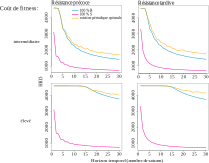
\includegraphics[width=1\linewidth]{fig5_1}
	  \caption[Rendement annuel moyen en fonction de l'horizon temporel pour les modèles avec résistance précoce et 
	  tardive]{Rendement annuel moyen ($\overline{HRD}$) en fonction de l'horizon temporel des rotations périodiques 
	  optimales (en jaune), ainsi que des stratégies résistantes (en bleu) et sensibles (en magenta) pures,  pour les 
	  modèles avec résistance précoce (\textbf{à gauche}) et tardive (\textbf{à droite}).}
	  \label{fig:compaR-hrd}
   \end{figure}
	
   \begin{figure}
	 \centering
	  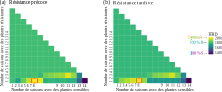
\includegraphics[width=1\linewidth]{fig5_2bis}		
	  \caption[Rendement annuel moyen de toutes les rotations périodiques sur un horizon de 15 ans pour les modèles 
	  avec résistance précoce et tardive]{Rendement annuel moyen ($\overline{HRD}$, gradient de couleur) de toutes les 
	  rotations périodiques sur un horizon de 15 ans,  avec en abscisse le nombre de saisons de plantes sensibles et en 
	  ordonnée celui de plantes résistantes (R), pour les modèles avec (\textbf{a}) résistance précoce  et (\textbf{b}) 
	  tardive. Les rendements des stratégies résistantes et sensibles pures, sont indiquées sur l'échelle de couleur. 
	  Ils sont sensiblement identiques pour les deux modèles. La stratégie encadrée en rouge correspond à la rotation 
	  périodique optimale.}
	  \label{fig:compaR-rotations}
   \end{figure}
	
	
	On constate que le type de résistance, précoce ou tardif, n'a quasiment aucun impact, ni sur le rendement annuel moyen, ni sur la stratégie périodique optimale, qui sur 15 ans est composée dans les deux cas d'une saison avec plantes résistantes suivie de cinq saisons avec plantes sensibles.
	
	Dans le modèle avec résistance tardive, on s'attendrait à ce que les nématodes avirulents, en pénétrant dans les racines de la plante résistante, induisent une immunité de la plante et ainsi la protègent partiellement des nématodes virulents. C'est le cas, mais ce phénomène est négligeable, car les nématodes avirulents ne peuvent pas se reproduire sur la plante résistante et leur population décroît alors rapidement. Sur la plante sensible, de par les coûts de virulence affectant les nématodes virulents, les nématodes avirulents prennent l'avantage.
	
\subsubsection{Durabilité des gènes majeurs précoces et tardifs}
	
	Nous avons ensuite comparé la durabilité (en nombre d'année) des deux résistances en fonction du coût de fitness efficace, défini en \eqref{eff_w} pour le modèle avec résistance précoce et de manière similaire (en remplaçant $w_{\beta}$ par $w_{\lambda}$) pour le modèle avec résistance tardive.
	
   \begin{figure}
	 \centering
	  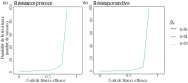
\includegraphics[width=1\linewidth]{fig5_3}		
	  \caption[Durabilité des résistances en fonction du coût de fitness efficace pour les modèles avec résistance 
	  précoce et tardive]{Durabilité des résistances en fonction du coût de fitness efficace $w$ pour les modèles avec 
	  résistance \textbf{(a)} précoce et \textbf{(b)} tardive.}
	  \label{fig:compaR-durab}
   \end{figure}
	 
	De nouveau, le type de résistance n'a pas d'impact sur les résultats (\autoref{fig:compaR-durab}). La résistance n'est  durable  que  pour de forts coûts de fitness. D'après la littérature, les résistances tardives sont connues pour être plus durables que les résistances précoces \cite{Castagnone-Sereno2002,Pegard2005,Djian-Caporalino2011,Barbary2014,Djian-Caporalino2014}.  Cette étude préliminaire suggère ainsi que la plus forte durabilité du gène de résistance tardive pourrait être liée non pas aux mécanismes de résistance seuls, mais à des coûts de fitness plus élevés par rapport au gène de résistance précoce.  Une explication plausible serait que le nématode a plus de \og serrures \fg{} à déverrouiller face à une plante avec une résistance tardive.
	 
	En conclusion, aucune  différence  entre les deux types de résistances n'a pu être observée dans cette étude, ni sur les rotations optimales et leur performances, ni sur leur durabilité, essentiellement parce que les nématodes avirulents ne peuvent pas se développer sur les plantes résistantes.
	
	
\subsubsection{Introduction d'un réservoir de plantes sensibles non cultivées} \label{sec:plante-reservoir}
	
	Nous avons donc poursuivi l'étude sur la durabilité en introduisant  un \og réservoir \fg{}  de plantes sensibles aux modèles de résistance tardive et précoce, présenté dans l'\Cref{annexeChap5}.
Ce réservoir correspond à des plantes sauvages, adventices ou à des débris de racines, présents toute l'année, mais ne présentant pas d'intérêt agronomique. C'est une situation qui  se rencontre dans de nombreux  systèmes de culture, notamment avec les virus \citep{Fabre2012}. Ce réservoir permet le maintien de nématodes avirulents dans la population globale, même lors d'une culture de plante résistante.
Dans le cas du modèle avec résistance tardive, une compétition avec les virulents pour les ressources de la plante pourrait être observée et fournir un effet bénéfique sur la durabilité des résistances. 
Notamment, le  maintien de variants avirulents dans la population grâce à la présence  d'un \og réservoir \fg{}  de plantes sensibles ne favorise pas la transmission de l'infection des nématodes virulents sur  des plantes résistante à \gls{HR} tardive car cette transmission se retrouve réduite à cause de la présence de nématodes avirulents qui occupent des sites nourriciers disponibles et immunisent la plante résistante.} Cela s'apparente au mélange de variétés (voir~\ref{durabilite_sub}.\ref{subsubsec:mel}).
	
   \begin{figure}
	 \centering 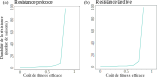
\includegraphics[width=1\linewidth]{fig5_4}
	  \caption[Durabilité des résistances en fonction du coût de fitness efficace pour les modèles avec résistance 
	  précoce et tardive en présence d'un réservoir]{Durabilité des résistances en fonction du coût de fitness efficace 
	  $w$ pour les modèles avec résistance \textbf{(a)} précoce et \textbf{(b)} tardive  en présence d'un réservoir de 
	  plantes sensibles non cultivées.}
	  \label{fig:compaR-durab}
   \end{figure}
	
	
	
	Une fois encore, nous n'avons pas observé de différences notables sur la durabilité entre les deux modèles de résistance (\autoref{fig:compaR-durab}). 
	
	Nous avons alors étudié l'influence de différents facteurs sur la durabilité : la taille du réservoir à l'équilibre ($S_{eq}$), qui était de 6~UR dans la~\autoref{fig:compaR-durab},  et pour le modèle avec résistance tardive, le taux de nécrose induit par une plante résistante pour bloquer un nématode avirulent après pénétration dans la racine. Plus précisément,   nous supposons  dans notre modèle de  résistance tardive qu'un nématode avirulent peut pénétrer
dans le système racinaire de la plante et induire des cellules géantes, mais ils sont interrompues 2 jours
après l'initiation de ces cellules géantes par les tissus nécrosés des racines de la plante \citep{Pegard2005}.  Le taux de nécrose ($1-\psi$) est  donc la perte d'une fraction de racine saine au niveau d'un site nourricier pour interrompre le développement d'un nématode avirulent.
	   
   \begin{figure}
	 \centering 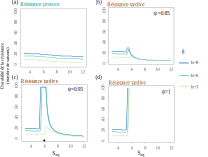
\includegraphics[scale=0.8]{fig5_5.pdf}
	  \caption[Durabilité des résistances en fonction de la taille du réservoir]{Durabilité des résistances en fonction 
	  de la taille du réservoir de plantes sensibles non cultivées $(S_{eq})$, pour différents taux de mutation ($
	  \delta$), pour les modèles avec résistance  \textbf{(a)} précoce et  \textbf{(b-d)} tardive avec différents taux 
	  de nécrose ($1-\psi$) induits par les nématodes avirulents dans la plante résistante.}
	  \label{fig:compaR-durab-Seq}
   \end{figure}
	
	
	
	Les résultats sont présentés \autoref{fig:compaR-durab-Seq}. La taille du réservoir de plantes sensibles non cultivées n'a quasiment pas d'effet sur la durabilité de la résistance précoce.
	
	En revanche, la taille du réservoir a un effet sur la résistance tardive, accentué pour de faibles taux de nécrose. Sans nécrose ($\psi=1$), cet effet est très bénéfique, mais seulement à partir d'un seuil donné. Cela peut s'expliquer ainsi : quand le réservoir est \og assez grand \fg{}, la population de nématodes avirulents peut se maintenir à une taille suffisante pour attaquer et immuniser les racines de la plante résistante. Sans nécrose induite par les nématodes avirulents dans la plante résistante, le rendement est alors optimal. La nécrose  qui se définie comme une perte ou destruction  d'une fraction de racine saine au niveau d'un site nourricier pour bloquer un nématode avirulent tempère, voire annule cet effet bénéfique : les attaques de la plante résistante par les nématodes avirulents favorisent certes l'immunité des racines, mais elles les détruisent aussi. La destruction de racines dans une saison a une influence sur la durabilité car elle se définit précisément : comme le nombre de saisons au bout duquel le déploiement de plantes résistantes engendre une perte de racines saines cumulées supérieure à 1\% par rapport à celles cumulées sur la saison initiale. C’est pourquoi la durabilité commence par augmenter avec la taille du réservoir,
puis chute.  Par exemple, si on considère la \autoref{fig:compaR-durab-Seq}c   la durabilité est de 17 saisons pour une taille de réservoir inférieur à $5,8$. À partir de ce seuil la résistance est extrêmement durable, c'est-à-dire que nous n'avons pas observé une perte de densités de racines saines cumulées supérieure à 1\% au moins sur 100 saisons par rapport à celles cumulées lors de la première saison. Mais cette durabilité chute pour une grande taille de réservoir. Au bout de deux saisons successives du déploiement de la résistance, nous avons observé  une perte de densités de racines saines cumulées supérieure à 1\% par rapport à celles obtenues lors de la première saison d'introduction de la résistance.
	 
	En conclusion, notre étude a permis de montrer l'importance d'une bonne compréhension des interactions hôte-pathogène afin de fournir une gestion plus durable des résistances. 
Bien que des expériences en laboratoire et en champs n'aient pas mis en évidence  de contournement  du  gène \textit{Me1} tardif du piment \citep{Djian-Caporalino2011, Djian-Caporalino2014} cela ne signifie pas qu'il ne  faut pas protéger cette résistance car tôt ou tard une évolution des pathogènes est possible \citep{Parlevliet2002}.  Il serait intéressant de confronter nos résultats théoriques à l'expérimentation, pour vérifier si un apport d'avirulents peut réduire le développement de nématodes virulents sur une plante résistante.
	
	
	 
\subsection{Résistance quantitative}
	
	La lutte génétique contre les nématodes à galle consiste principalement à utiliser des gènes majeurs de résistance (résistance qualitative ou totale). Ce n'est que  très récemment que quatre \glspl{QTL} ont été identifiés dans le piment \citep{Barbary2016}. Ces \glspl{QTL} réduisent le nombre 
des masses d'œufs produites sur les racines de cultivars résistants \citep{Barbary2014} et donc
peuvent réduire le risque d'émergence et de sélection ultérieure de nématodes virulents. \citet{Sanchez-Solana2017} ont également fait état de l'existence d'une résistance quantitative vis-à-vis des nématodes à galles chez les variétés de piments (\textit{Capsicum}) et ont conclu que cette résistance peut éviter l'émergence et éviter la sélection de pathogènes non adaptés, lui conférant une certaine durabilité à la fois par elle-même et en combinaison avec les principaux gènes \textit{Mi}
	
	Notre modèle met en œuvre une résistance qualitative, car il s'appuie sur l'exemple de la tomate, dont le gène \textit{Mi-1} confère une résistance totale \citep{Milligan1998} et est le seul gène présent actuellement dans les variétés commercialisées.
Nos travaux se concentrent sur des résistances qualitatives qui agissent comme un
mécanisme de « tout ou rien », qui implique une reconnaissance du gène d’avirulence du parasite par le
gène de résistance de la plante, qui bloque le parasite. Du fait que des \glspl{QTL} contrôlant différents traits de vie aient été identifiés dans les piments résistants, il nous semble intéressant d’exploiter  les résistances quantitatives comme c'est le cas dans de nombreux pathosystèmes (voir section \ref{sec:quantitatives}).
	
	
	Notre cadre de modélisation est assez souple pour  nous permettre d'étudier une résistance  polygénique partielle.
	Son intégration dans notre modèle peut se faire en modifiant la valeur de certains paramètres, en particulier le succès de l'infection, qui ne serait alors plus du tout ou rien mais qui pourrait prendre des valeurs intermédiaires. Cela rejoindrait par exemple les travaux de  \citet{Leonard1977} ou  \citet{Tellier2007, Tellier2011}, dans lesquels
l'efficacité de la résistance contre les agents pathogènes avirulents  peut prendre un continuum  de valeurs.
On peut citer également les travaux de \citep{Rousseau2019} qui ont étudié la durabilité d'un gène majeur de résistance lorsqu’il est en présence d’un fond génétique conférant un niveau de résistance quantitative dans le cas des virus. Ces travaux se concentrent sur des résistances qui agissent sur des traits tels que la capacité à infecter les plantes porteuses du gène majeur de résistance,
la taille efficace de population virale, ainsi que le coefficient de sélection et l’accumulation virale.
Dans notre cas, des traits du pathogène pourraient également être modifiés, comme par exemple le taux de reproduction et le taux d'infectivité, en fonction de la résistance déployée.
	
\subsection{Rotations et pyramidage}
	
	Nous avons étudié dans cette thèse des stratégies d'alternance entre plantes sensibles et plantes porteuses d'un gène de résistance majeur. En termes de perspectives, il serait pertinent d’explorer, à partir de ce cadre de modélisation, d'autres scénarios de déploiement des résistances fondés sur des rotations et/ou du pyramidage de gènes. En effet, les mélanges variétaux et mosaïques, autres stratégies de déploiement (voir section~\ref{durabilite_sub}), semblent peu efficaces pour protéger les cultures des nématodes, notamment à cause de la faible dispersion de ce parasite \citep{Djian-Caporalino2014}.
Parmi les stratégies d'intérêt important, nous pouvons citer : (i) l'alternance dans le temps de deux gènes majeurs de résistance ; (ii) le pyramidage de deux gènes majeurs ou l'introgression d'un gène majeur dans un fonds génétique avec une résistance quantitative ; (iii) l'alternance entre une variété portant deux \glspl{gene R} pyramidés et des variétés porteuses d'un des deux gènes. Notre modèle permettrait, dans chacun de ces cas, de déterminer des stratégies de déploiement optimisant l'efficacité et la durabilité des résistances. Le but serait de fournir des recommandations sur quelles résistances utiliser et comment les déployer, selon différents facteurs tels que l'intensité de l'infestation, la pré-existence de nématodes virulents, \textit{etc.} En particulier, on pourrait déterminer quand l’utilisation d’un seul gène de résistance est plus efficace, ou dans quelles conditions le pyramidage des gènes
peut être défaillant.  On pourrait déterminer quelles résistances quantitatives sont les plus
bénéfiques à combiner avec un gène majeur et lesquelles au contraire il pourrait être moins intéressant d’associer.
\citet{Rimbaud2018a} ont en effet montré que dans le cas de la rouille sur des céréales, il était parfois préférable d’alterner plutôt que pyramider deux gènes majeurs de résistance, en particulier s'ils avaient déjà été contournés auparavant.
	
\section{Acceptabilité des stratégies par les agriculteurs}
	
	Dans cette étude nous avons proposé des stratégies  de rotation  alternant des plantes résistantes et sensibles d'une même espèce.  
	
	Nous avons montré que pour maximiser le rendement annuel moyen sur le long terme,  il était préférable d'utiliser de faibles ratios de plantes résistantes  (voir section~\ref{sec:discussion-lowratio}). À titre d'exemple, pour un horizon temporel de 15 ans, les meilleures rotations en termes de rendement moyen ne mettent en œuvre que 20 à 27\% de plantes résistantes. De plus, ces stratégies sont robustes aux variations et incertitudes sur les valeurs des paramètres, ainsi qu'aux variations des  taux d'infestations des sols (voir section~\ref{sec:discussion-OptRot-in-practice}).
	
	Cependant,  ces stratégies se heurtent à deux principales limites en matière d'acceptabilité par les agriculteurs.  Premièrement, ces stratégies  peuvent  entraîner de fortes variations de rendement au fil du temps. Des années à faibles rendements peuvent se succéder et entraîner des pertes économiques conséquentes pour les agriculteurs. Deuxièmement, les agriculteurs sont peu enclins à utiliser une variété sensible quand il existe une variété résistante de la même plante. Ainsi, les agriculteurs dans le sud de la France acceptent l'alternance de tomates résistantes et de melons sensibles, mais plus difficilement l'alternance de tomates résistantes et sensibles. Cette stratégie pourrait être mieux adaptée chez les agriculteurs au Maroc car ce que nous avons modélisé est pratiqué dans ce pays. 
Nous pouvons donc proposer les meilleures stratégies  possibles pour gérer les nématodes à galles sur le long terme mais,  si elles se heurtent à un problème d'acceptabilité, elles ne seront pas appliquées.
	
	Pour pallier ces problèmes d'acceptabilité, il existe plusieurs solutions. Elles consistent d'abord à réconcilier l'usage des stratégies classiquement  utilisées à court terme par les agriculteurs (culture d'une variété agronomique résistante) et celles recommandées pour préserver un rendement moyen intéressant à long terme. Une de ces solutions serait  de tirer profit de la faible mobilité des nématodes afin de proposer des rotations de cultures  asynchrones dans différentes parcelles agricoles. Pour ce faire, il faudrait décaler d'une année ou plus la stratégie optimale dans les différentes parcelles de l'exploitation. Après plusieurs années consécutives de cultures sensibles, les rendements baissent notablement, puis augmentent à nouveau quand la résistance est introduite. Idéalement, il faudrait qu'au moins une parcelle soit cultivée avec des plantes résistantes chaque année. Mais une attention particulière devrait être portée à la mise en œuvre  de bonnes pratiques agricoles  pour éviter la contamination entre les parcelles, essentiellement liées au travail du sol. À l'échelle de l'exploitation, cela permettrait de lisser les variations saisonnières de rendement et d'assurer un revenu plus stable aux agriculteurs.  Pour aller plus loin,  il faudrait également viser  une optimalité  du déploiement spatio-temporel des rotations, tout en respectant des contraintes socio-économiques de rentabilité et de maintien d’un niveau de revenu
minimal au long des saisons. 
	
	Enfin, au-delà de l'asynchronisation des systèmes de culture décrite ci-dessus et des différentes rotations de résistances pyramidées ou non présentées précédemment, une perspective de notre travail consisterait à élargir nos rotations à différentes espèces maraîchères, plus ou moins bons hôtes pour les nématodes à galles.  
Des producteurs du sud de la France ont mis en place un réseau pour mieux gérer la résistance et contrôler les nématodes à galles à travers différents projets (projet Gedunem 2012-2016,
Projet européen GONEM 2018-2021). Par exemple,  la tomate porteuse du gène \textit{Mi-1}  ou le poivron porteur du gène \textit{Me-3} peut être cultivé tous les deux ans, en rotation avec des cucurbitacées en été et des salades en hiver \citep{Talavera2009, Gine2017}.
Ces systèmes, très similaires à notre étude, pourraient être modélisés et étudiés dans le but de déterminer des stratégies  optimales de  déploiement de la résistance des plantes. Les recommandations issues de ces travaux pourraient être  mieux acceptées par les agriculteurs impliqués dans ces différents projets, puisqu'ils implémentent déjà  des stratégies similaires à court et moyen termes dans leurs propres parcelles. % Pour contribuer à améliorer l'acceptabilité des stratégies théoriques proposées et face aux forces en présence, un dialogue entre les scientifiques et les professionnels de l'agriculture doit être omniprésent pour passer d'une agriculture traditionnelle vers une agriculture plus durable, sociale, environnementale et économiquement stable.
	
	%%% Local Variables:
	%%% mode: latex
	%%% TeX-master: "these_main"
	%%% End:
